This sections evaluates the performance of proposed methodology in estimating correspondences of human poses in-the-wild. Results for quantitative an qualitative experiments are reported. Experiments \ref{exp:internal} investigate the accuracy of estimating dense correspondences of non-rigid deformable objects, and the impact of annotating outlines of human poses instead of annotating skeletons. Experiments \ref{exp:benchmark} compare the joints localisation accuracy of our skeleton prediction from outline fitting with respect to that of state-of-the-art human pose estimation algorithms in-the-wild. Note that all results reported in this section were obtained by fitting Patch AAM using the fast version of the Simultaneous Inverse Compositional algorithm (Fast-SIC) originally proposed by the authors of \cite{Papandreou2008}. For further experimental results and visualisations please refer to our supplementary material.


\subsection{Databases \& Error Metrics}
There are significant numbers of datasets exist for human pose estimation, where FLIC\cite{sapp2013modec}, BBC Pose\cite{pfister2015flowing}, Fashion Pose\cite{dantone2013human} and MPII\cite{andriluka14cvpr} attracted most public attention. In our work, we reported our performance comparison on BBC Pose Dataset\cite{pfister2015flowing}, which has relatively most consistent skeleton annotation among the others.

\begin{figure}[t!]
    \centering
    % \begin{subfigure}[b]{0.05\textwidth}
    %         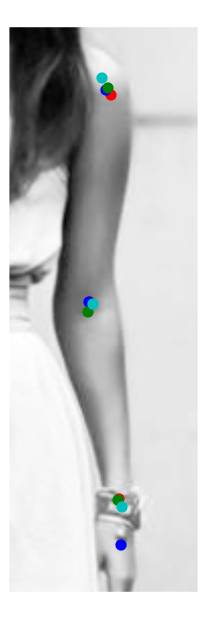
\includegraphics[width=\textwidth]{resources/Fig_Variance/image_0}
    % \end{subfigure}
    % \hfill
    \begin{subfigure}[b]{0.08\textwidth}
            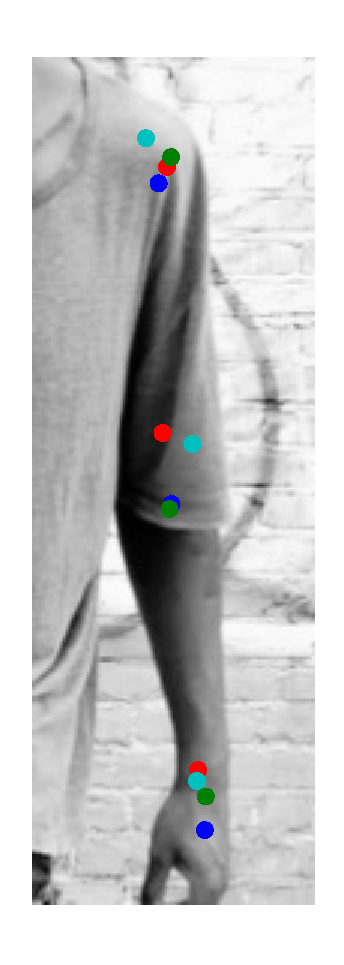
\includegraphics[height=5.5cm]{resources/Fig_Variance/image_1}
    \end{subfigure}
  	\hfill
    \begin{subfigure}[b]{0.08\textwidth}
            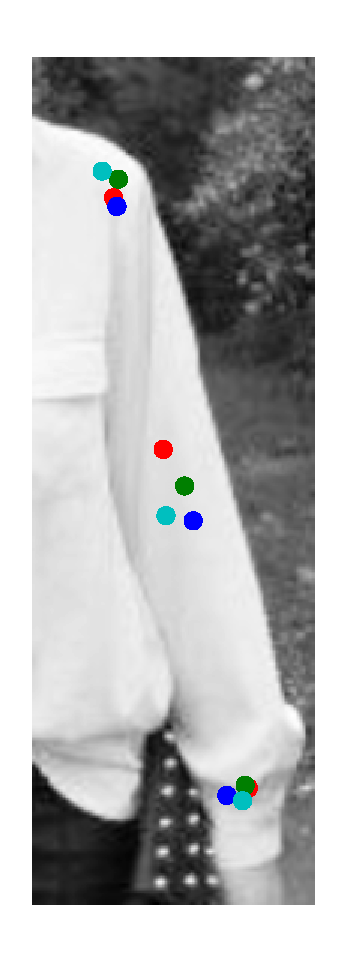
\includegraphics[height=5.5cm]{resources/Fig_Variance/image_2}
    \end{subfigure}
    \hfill
    % \begin{subfigure}[b]{0.07\textwidth}
    %         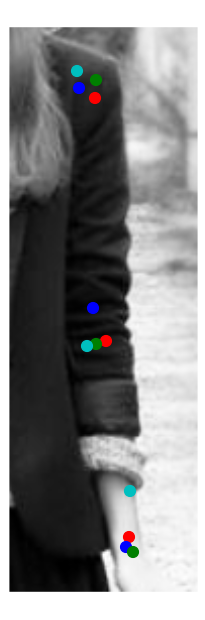
\includegraphics[height=4.8cm]{resources/Fig_Variance/image_3}
    % \end{subfigure}
    % \hfill
    \begin{subfigure}[b]{0.08\textwidth}
            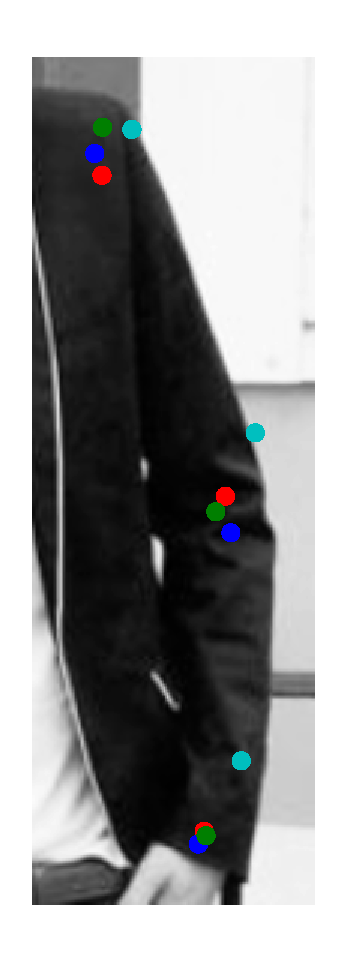
\includegraphics[height=5.5cm]{resources/Fig_Variance/image_4}
    \end{subfigure}
  	\hfill
    % \begin{subfigure}[b]{0.05\textwidth}
    %         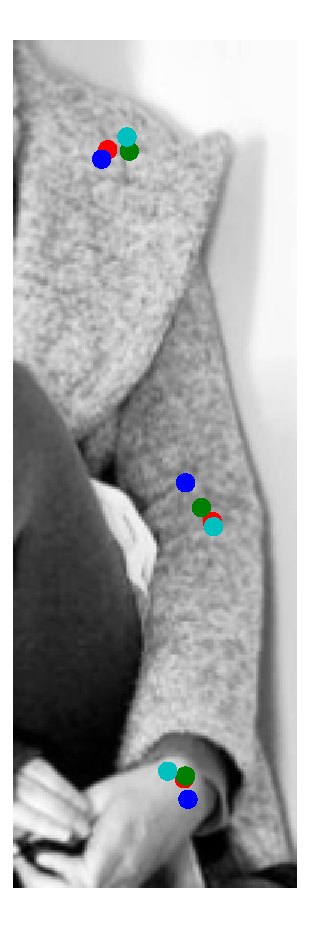
\includegraphics[width=\textwidth]{resources/Fig_Variance/image_5}
    % \end{subfigure}
    % \hfill
    \begin{subfigure}[b]{0.08\textwidth}
            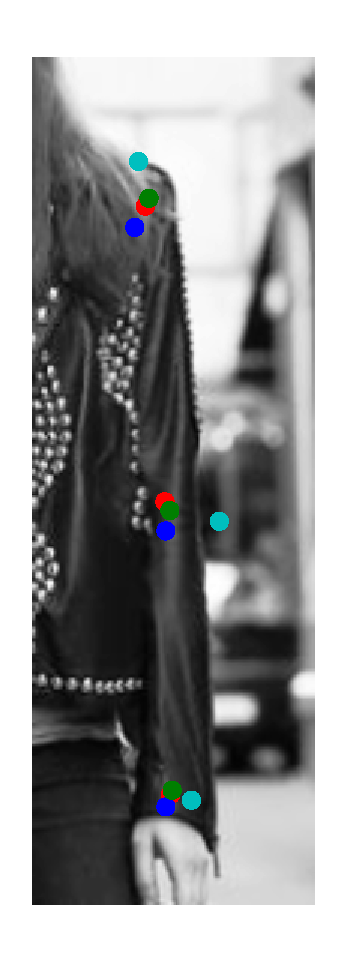
\includegraphics[height=5.5cm]{resources/Fig_Variance/image_6}
    \end{subfigure}
    \hfill
    \begin{subfigure}[b]{0.125\textwidth}
            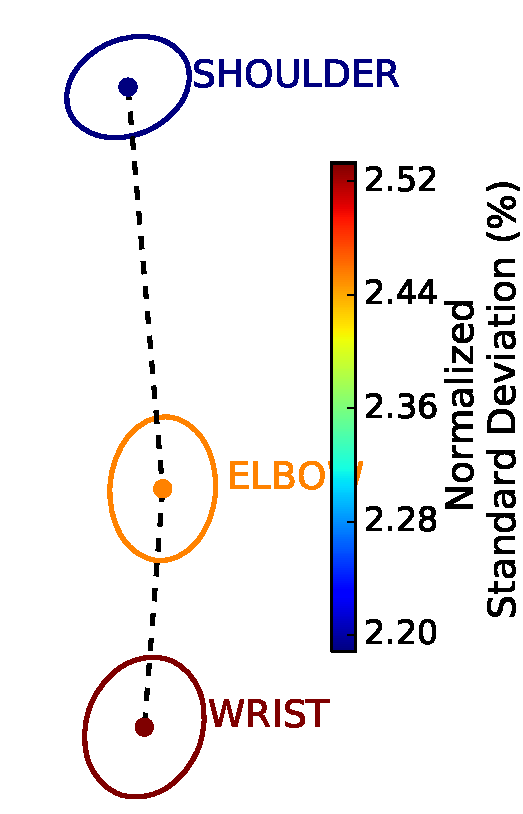
\includegraphics[height=5.5cm]{resources/Fig_Variance/variances}
    \end{subfigure}
    \caption{Exemplar human pose annotation for left arm among four annotators. Large variance shows the difficulties of have consistent landmarks. Figure best viewed by zooming in.}
    \label{fig:variance}
\end{figure}

The training of dense Active Appearance Models (dAAMs) for upper body involves manual outline annotation from a combination of datasets, including H3D \cite{PoseletsICCV09}, Microsoft COCO \cite{lin2014microsoft}, MPII \cite{andriluka14cvpr}, Fashion Pose \cite{dantone2013human}, FLIC \cite{sapp2013modec} and BBC Poses \cite{pfister2015flowing}. The training set contains 891 training images from where 500 are annotated with outline manually. A dAAMs is built from 500 training images thereby produces dense correspondences for generating sparse outline annotation (29 landmarks). A Patch AAM is build from sparse annotations before fitting to 391 images. Manual minor correction are required for putting those fitted image to training set. The final Patch AAM is built from 891 images and validated on validation set given by BBC Pose.

In order to compare with current state-of-the-art human pose estimation on BBC Pose, we uses same error metric as BBC Poses does, which normalises testing images to have height of 256 pixels. Performance measure of experiments in this paper are plot with Cumulative Error Distribution (CED) curve, where graph shows accuracy against distance from ground truth in pixels on normalised images.

\subsection{Arm Pose Estimation}
\label{exp:benchmark}
Two experiments are undertaken in this section: 1) presenting training classic patch AAM from outline annotation provides remarkable joints estimation; 2) supporting outline annotation by comparing with training classic patch AAM from joint annotation .

First experiment presented the accuracy of predicting joints positions from establishing dense correspondences with outline fitting. We build patch AAM using 891 training hand images from a combination of datasets, where each image has 29 landmarks annotated alone its boundary. SIFT \cite{PoseletsICCV09} feature is used from image representation for our model. Model fitting is initialised based on current state-of-the-art human pose estimation algorithms on BBC Pose dataset. Results for this experiment are reported over 1000 testing images BBC Pose Provided, which human upper-body pose are landmark with 7 points on skeleton. For our model, joints are projected from the dense correspondence generated from our proposed method.

Second experiment investigates the disadvantages of using skeleton annotation. We build patch AAM on joints with same training data and with SIFT representation. Both models are fine-tuned on BBC Pose validation set. The fitting procedure is performed under exactly same condition, e.g. same testing set and initialisation position. 

CED Curves for both experiments are shown in Figure \ref{fig:hand_benchmark} while fitting statistics are shown in supplementary material. Results show that, for first experiment, the fitting accuracy achieved by our method outperformed current state-of-the-art algorithms. In particular, our method improves performance of current best method \cite{pfister2015flowing} by a notable amount (9\% with error less than 6pt) on wrist, as well as marginal improvement on elbow estimation. While for second experiment, patch AAM trained with outline significantly outperforms path AAM trained with joints as we expected. Note that path AMM trained with Joints still comparable even marginally better than recent algorithms.

\begin{figure}[b!]
    \centering
    \includegraphics[width=\columnwidth]{resources/HandBenchmark/legend}
    \\
    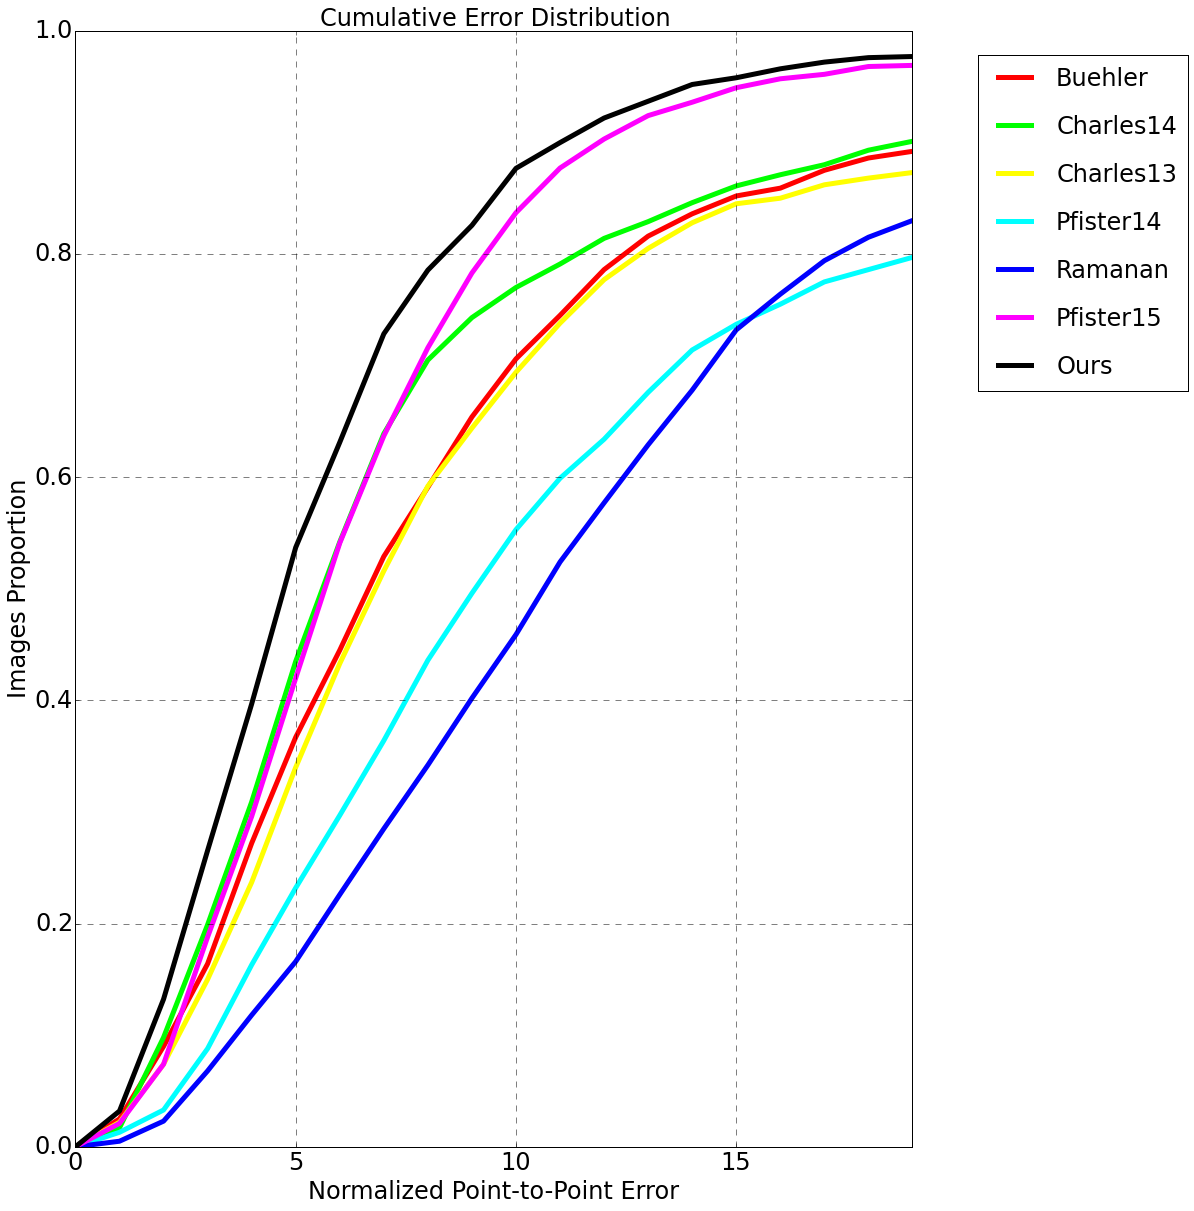
\includegraphics[width=0.48\columnwidth]{resources/HandBenchmark/wrist}
    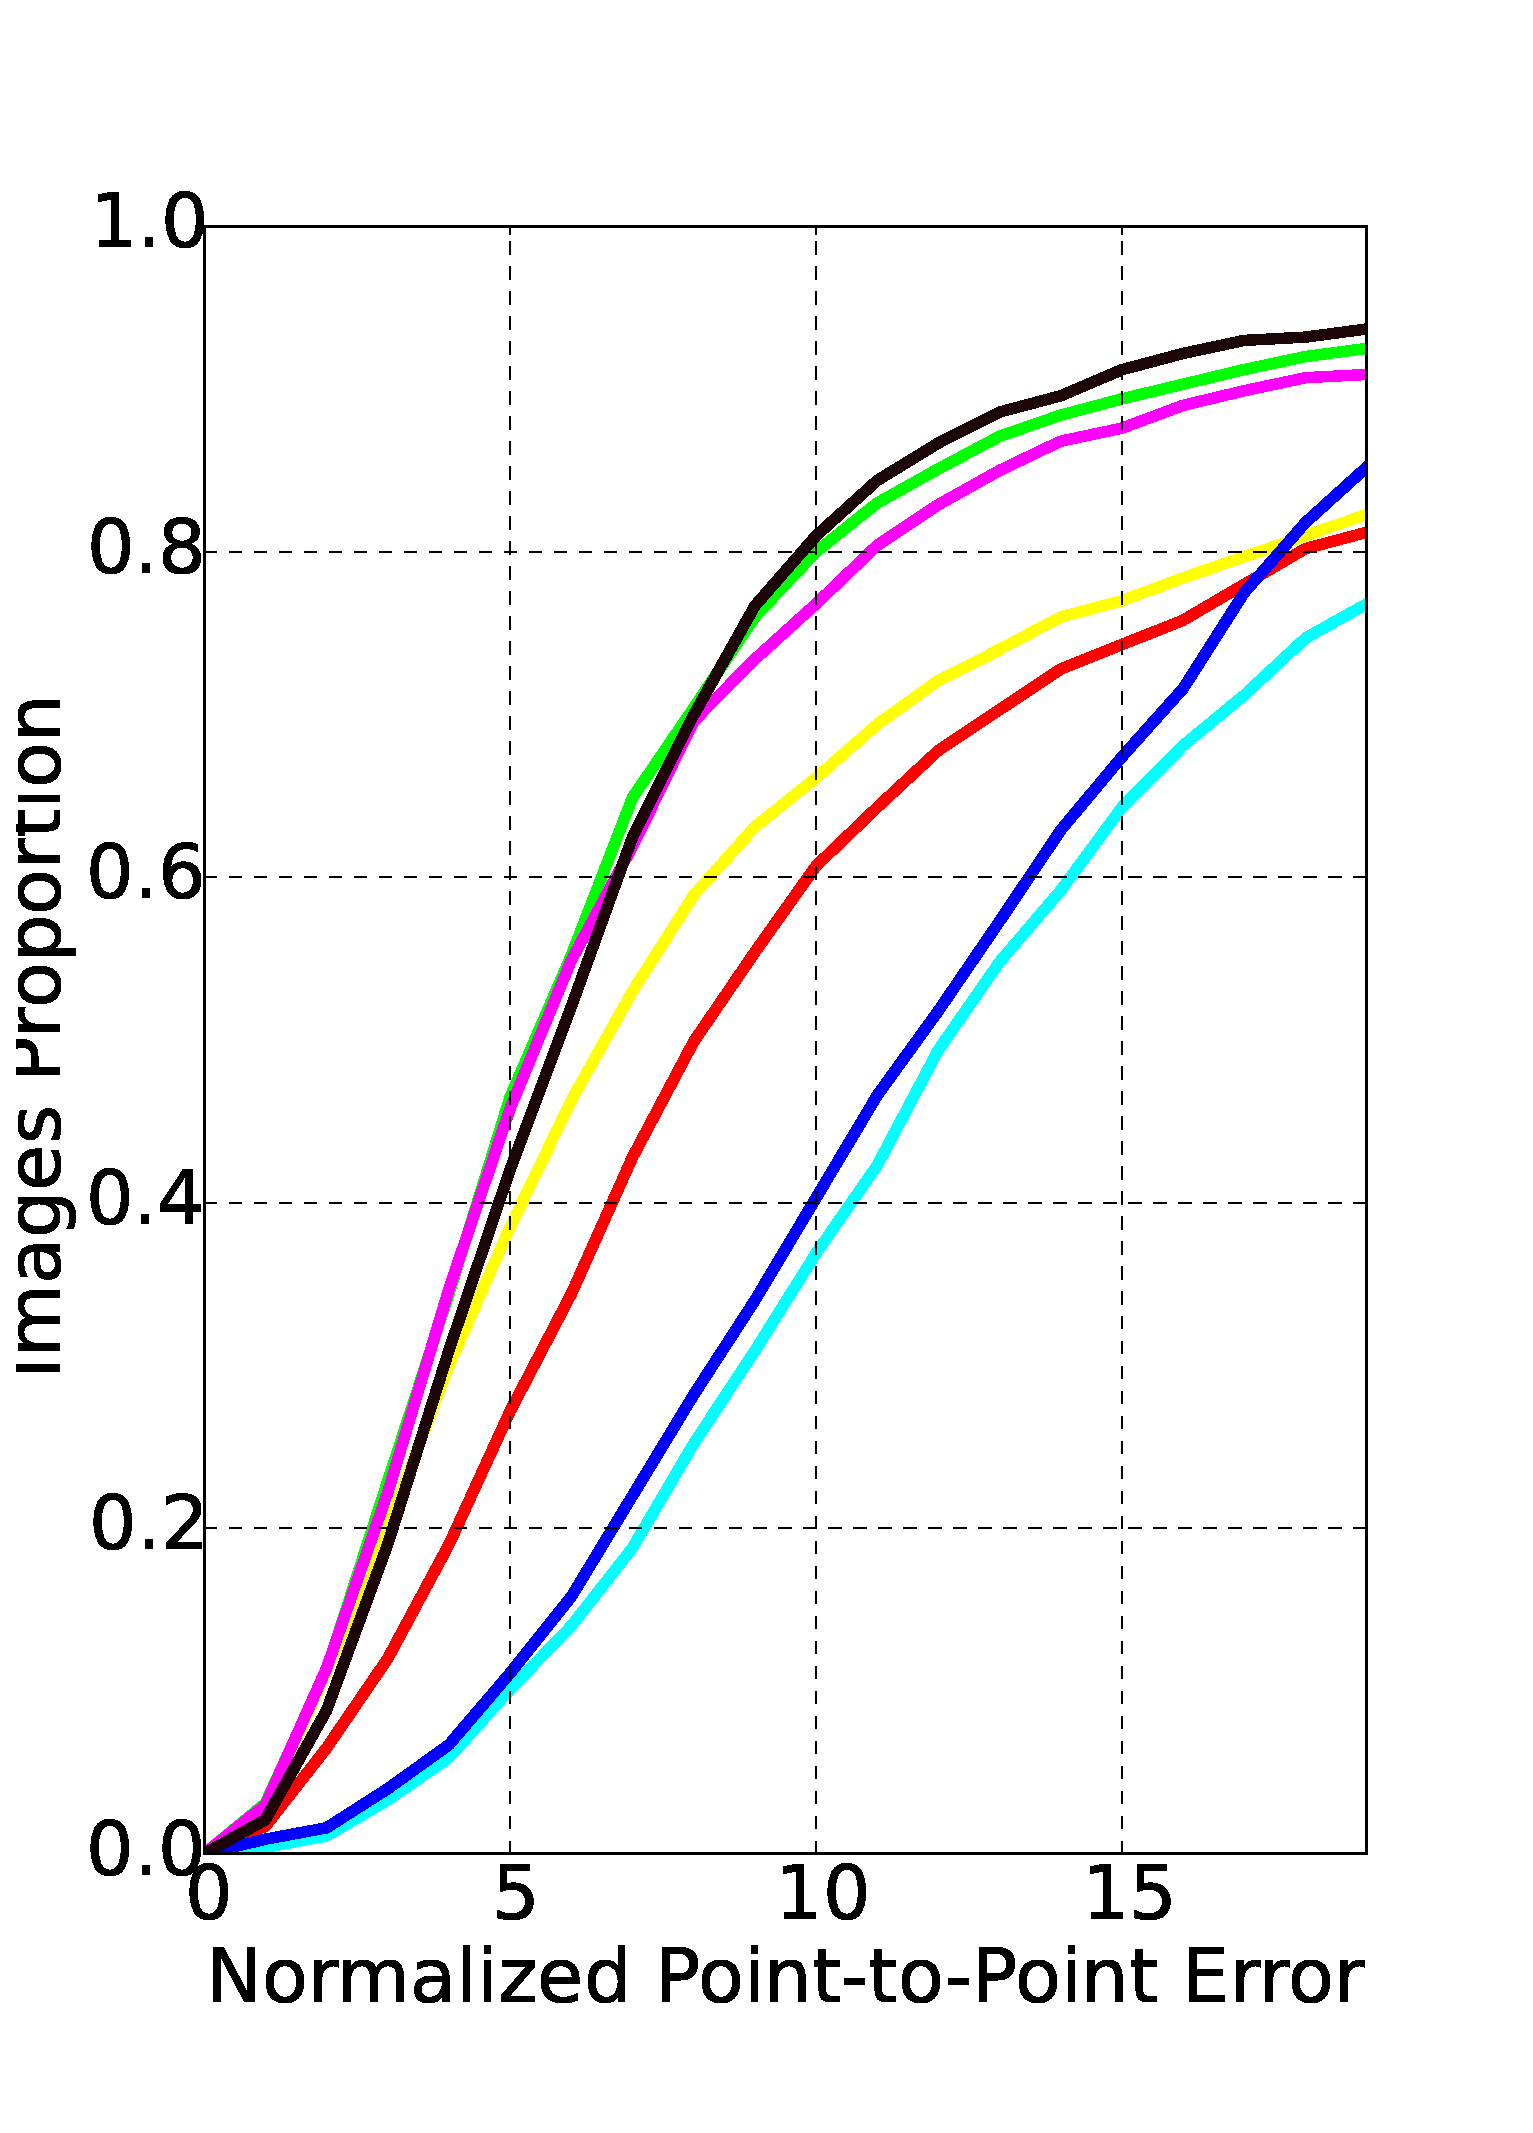
\includegraphics[width=0.48\columnwidth]{resources/HandBenchmark/elbow}
    \caption{CEDs over skeleton landmarks on BBC Pose database for experiment \ref{exp:benchmark}}
    \label{fig:hand_benchmark}
\end{figure}


% \begin{table}[b!]
%     \small
%     \centering
%     \begin{tabular}{|l|c|c|c||c|c|c|}
%         \hline
%                             & \multicolumn{3}{c||}{Wrist} & \multicolumn{3}{c|}{Elbow}\\
%         \hline
%         \emph{Method}       & \emph{mean} & \emph{std} & $\leq 6pt$ & \emph{mean} & \emph{std} & $\leq 6pt$\\
%         \hline\hline
%         Buehler             & 12.08    & 19.94        & 44.5\%       & 12.94    & 14.65        & 34.4\%\\
%         Charles14           & 11.81    & 20.89        & 54.2\%       &  8.30    & 11.00        & \textbf{55.2\%}\\
%         Charles13           & 13.78    & 22.39        & 43.3\%       & 13.17    & 18.74        & 46.3\%\\
%         Pfister14           & 14.69    & 17.89        & 29.7\%       & 14.60    & 10.59        & 14.0\%\\
%         Ramanan             & 15.59    & 19.04        & 22.6\%       & 15.53    & 10.82        & 15.8\%\\
%         Pfister15           & 7.62     & 11.04        & 54.1\%       &  8.84    & 11.44        & 54.9\%\\
%         \hline\hline
%         Ours                & \textbf{6.71}& \textbf{10.90}   & \textbf{63.1\%}       & \textbf{8.20}     &  \textbf{10.54}        & 52.1\%\\
%         \hline
%     \end{tabular}
%     \caption{Fitting statistics on BBC Pose database for experiment \ref{exp:benchmark}}
%     \label{tab:hand_benchmark}
% \end{table}


\subsection{Non-rigid Object Alignment In-the-wild}
\label{exp:daam_benchmark}
\begin{figure}[b!]
    \centering
    \includegraphics[width=\columnwidth]{resources/DAAMBenchmark/legend}
    \\
    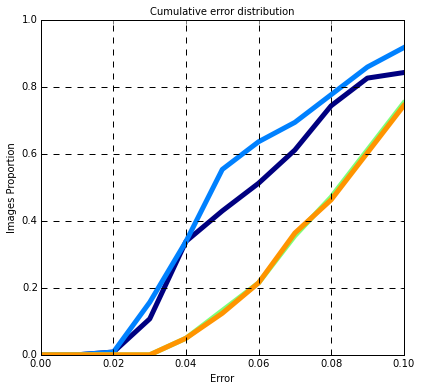
\includegraphics[width=0.48\columnwidth]{resources/DAAMBenchmark/face}
    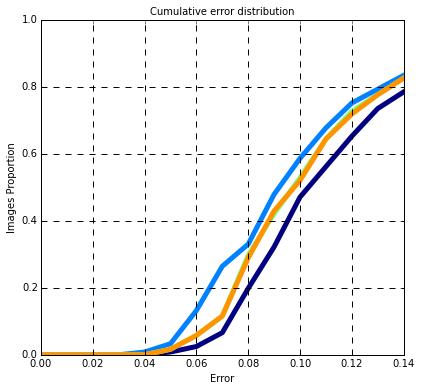
\includegraphics[width=0.48\columnwidth]{resources/DAAMBenchmark/ear}
    \caption{CEDs of faces and ears fitting performance for experiment \ref{exp:daam_benchmark}}
    \label{fig:daam_benchmark}
\end{figure}


This experiment compares the fitting accuracy of our dAAMs versus the one of classic AAM on the problem of nonrigid face and ear alignment in-the-wild. 

For face experiment, both models were built using the 811 training images of the Labelled
Faces Parts in-the-Wild (LFPW) \cite{Asthana2014} database. Classic AAM were built from 68 point landmark annotations using the standard procedure described in \cite{Cootes2001,Matthews2004}; piecewise affine was used as their motion model. Our dAAMs were built as the pipeline proposed. Results for this experiment are reported over the 224 testing images of the LFPW database using again 68 point ground truth landmark annotations. For this experiment, we report results using pixels intensities (INT) for both models. 

For ear experiment, we studied the feasibility of building and fitting statistical deformable models that capture the variability of the human ear. To this end, we collected 605 high resolution images of ears in unconstrained scenarios and annotated them using both a newly defined 55 point annotation scheme for ears and the curve annotations proposed in this paper. Examples of these two type of ear annotations are shown in Figure \ref{fig:intro}. We randomly split the previous database into two disjoint sets of training (500) and testing (105) images. Both models were built using the 500 images training set and their fitting accuracy evaluated on the 105 images of the testing set. Note here that we used the same procedures to build the models as for faces and same error metric for evaluation.

CED Curves for this experiment are shown in Figure \ref{fig:daam_benchmark}. We can readily observe that the accuracy achieved by ear models, in terms of the previous normalized point-to-point error measure, is lower than the one achieved by face models. This result is expected due to the more complex structure of the ear shape. Through visual inspection we determined that fitting errors below 0.1 for ears typically look plausible under the previous error measure where fitting errors below 0.6 for faces. Results show that, for this experiment, the fitting accuracy achieved by our dAAMs is marginally better to the one achieved by classic AAMs using intensity representations. In fact, classic AAM fail to improve the accuracy of the original initialisation on ears. Therefore the propose pipeline is capable of dealing with the complex structure of non-rigid shapes and learn dAAMs from simple curve line annotations that can compete and even surpass (in the case of a simple pixel intensity image representation) classic AAM, build from carefully annotated point landmarks, is quite remarkable.

\subsection{Annotation Correction}
\label{exp:qualitative}


\begin{figure}[b!]
    \centering
    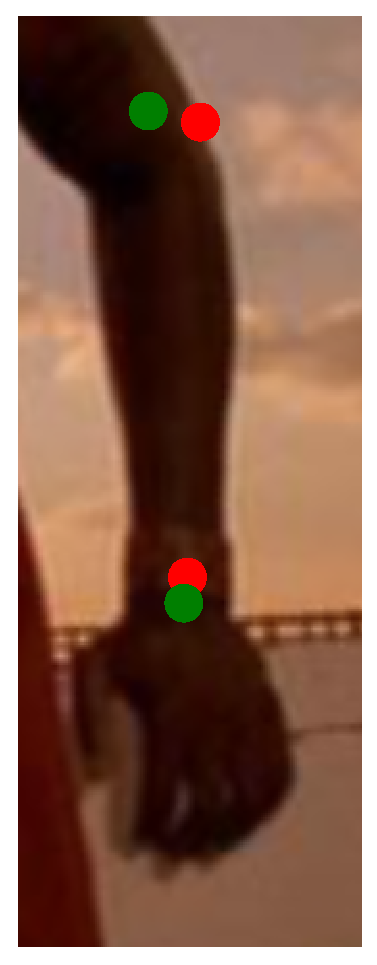
\includegraphics[height=0.3\columnwidth]{resources/Fixing/fix_3}
    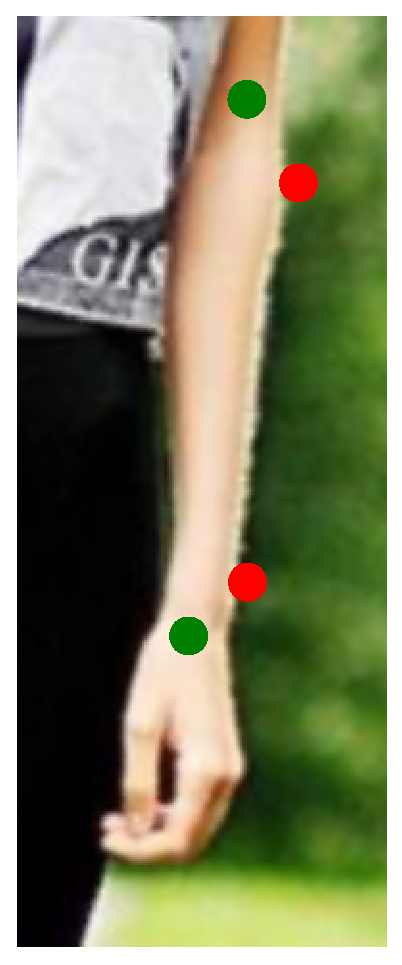
\includegraphics[height=0.3\columnwidth]{resources/Fixing/fix_5}
    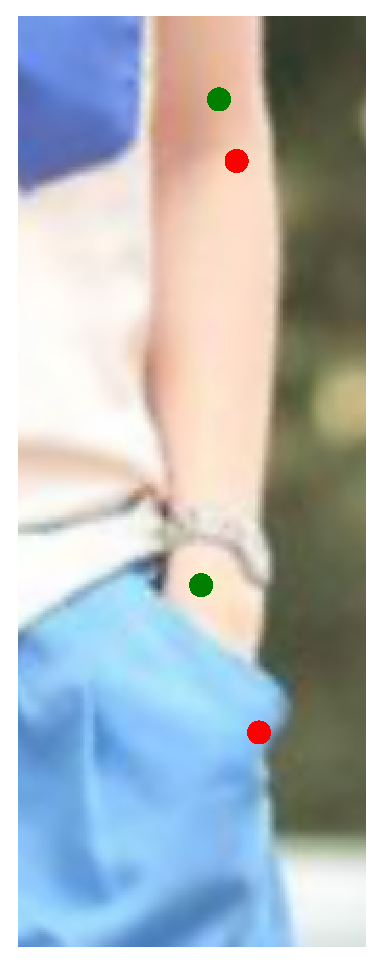
\includegraphics[height=0.3\columnwidth]{resources/Fixing/fix_6}
    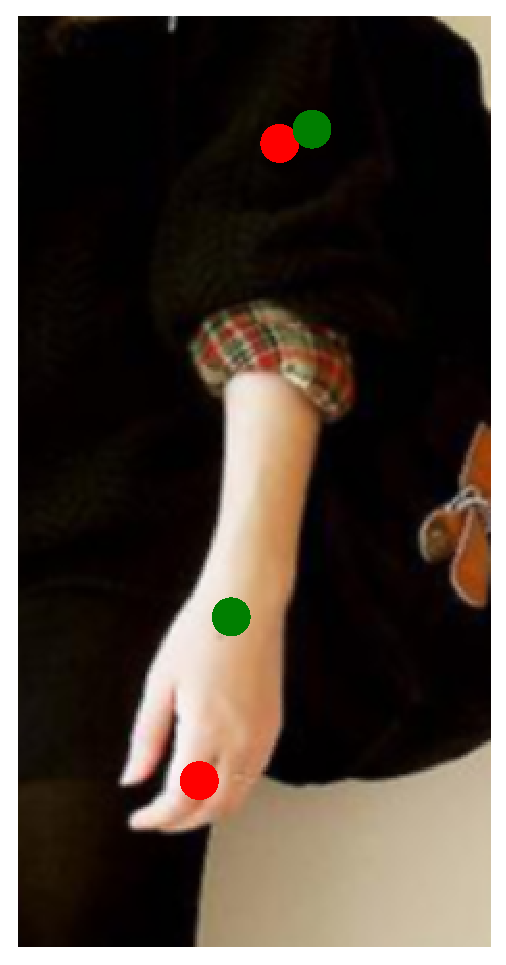
\includegraphics[height=0.3\columnwidth]{resources/Fixing/fix_7}
    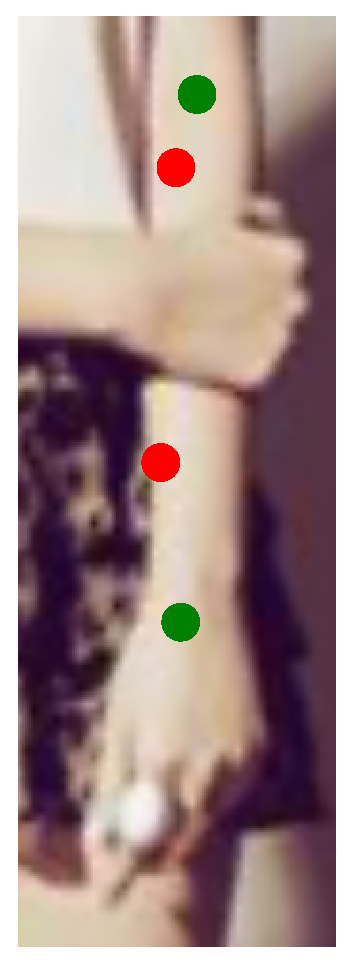
\includegraphics[height=0.3\columnwidth]{resources/Fixing/fix_8}
    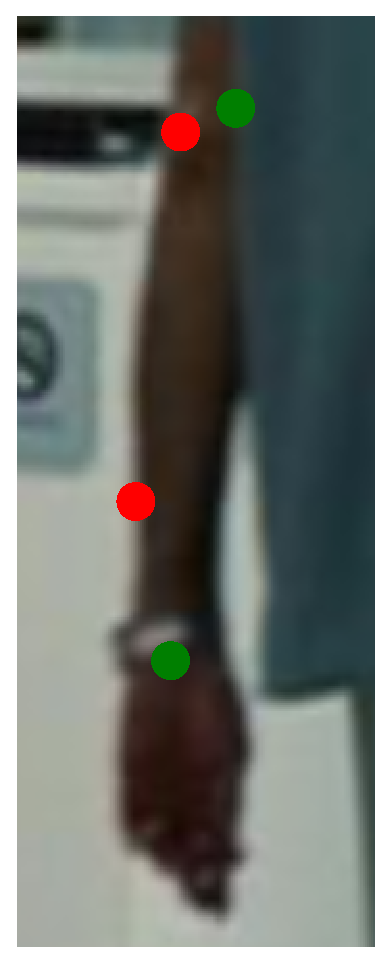
\includegraphics[height=0.3\columnwidth]{resources/Fixing/fix_9}
    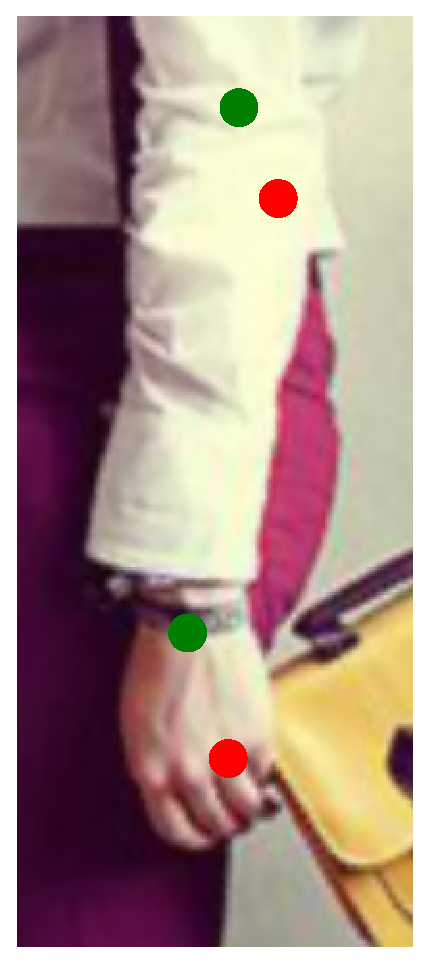
\includegraphics[height=0.3\columnwidth]{resources/Fixing/fix_10}
    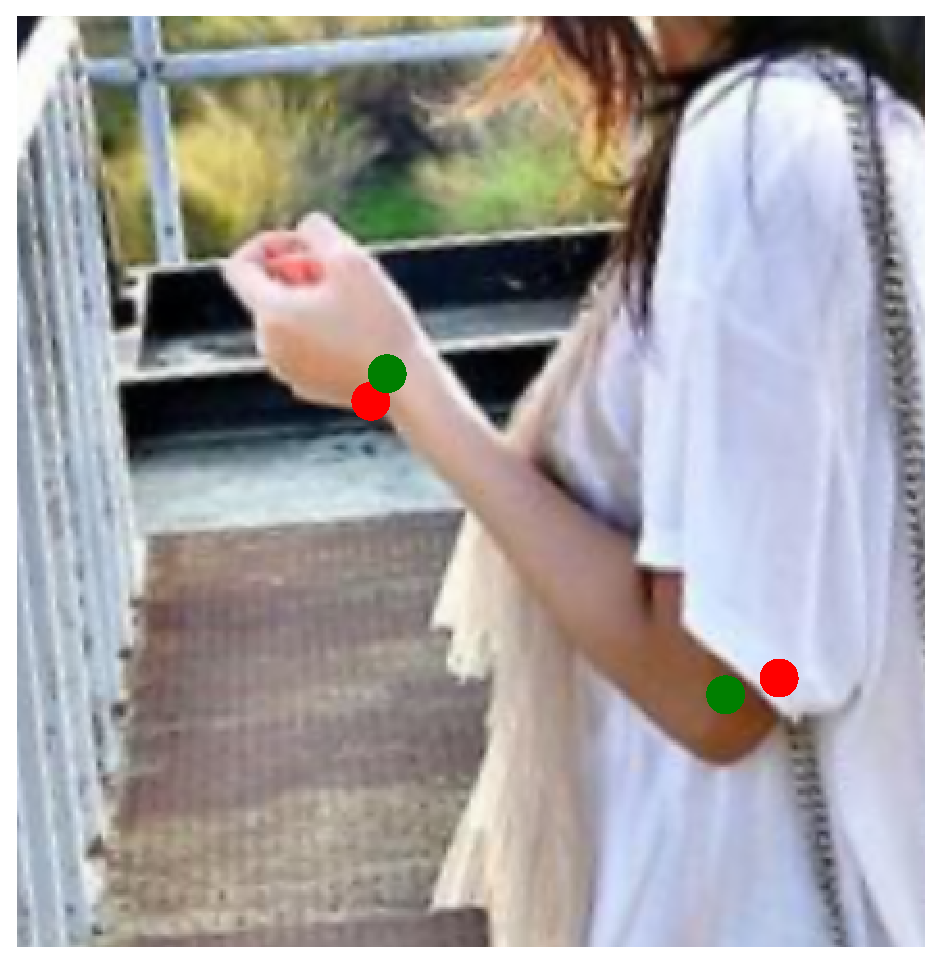
\includegraphics[height=0.3\columnwidth]{resources/Fixing/fix_11}
    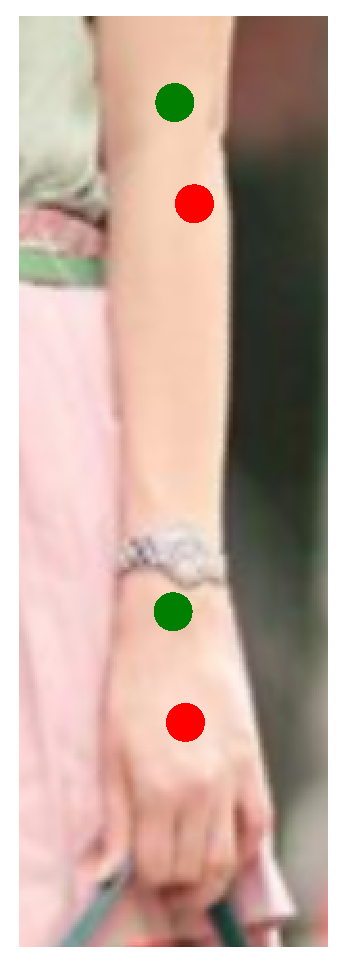
\includegraphics[height=0.3\columnwidth]{resources/Fixing/fix_12}
    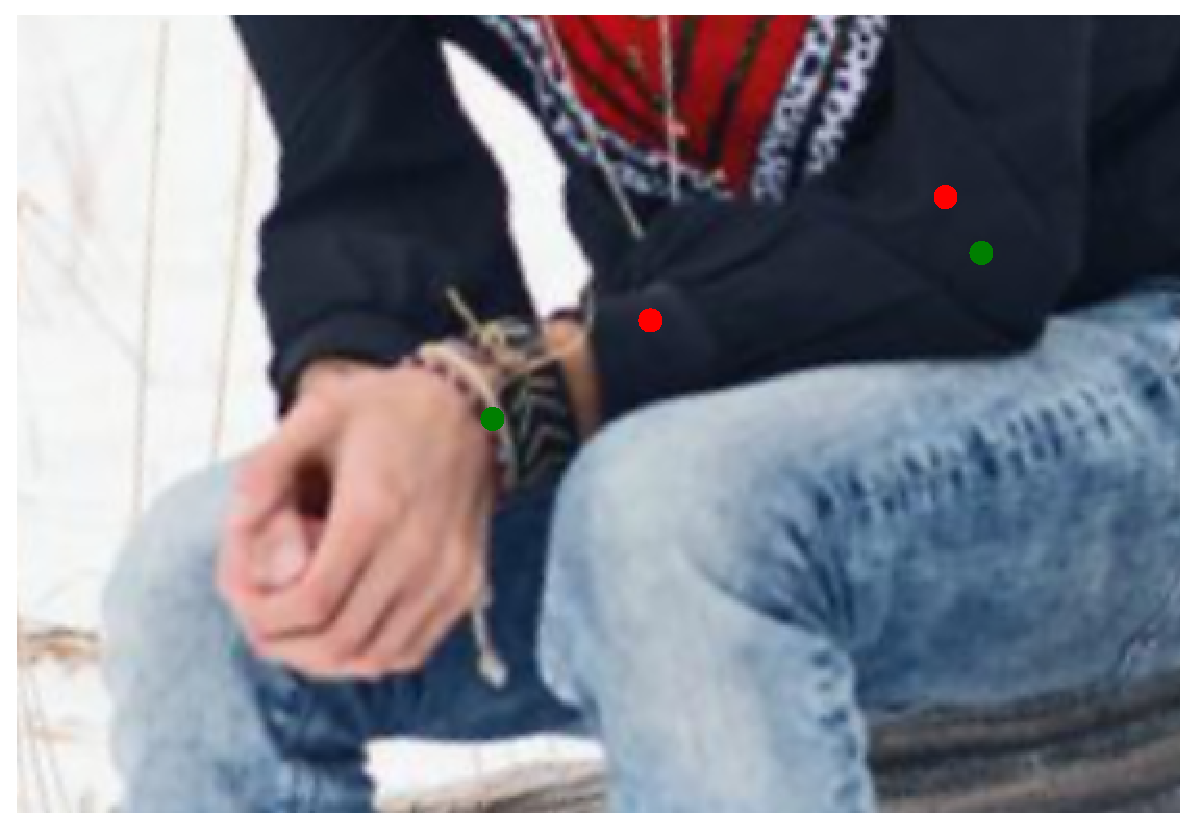
\includegraphics[height=0.3\columnwidth]{resources/Fixing/fix_13}
    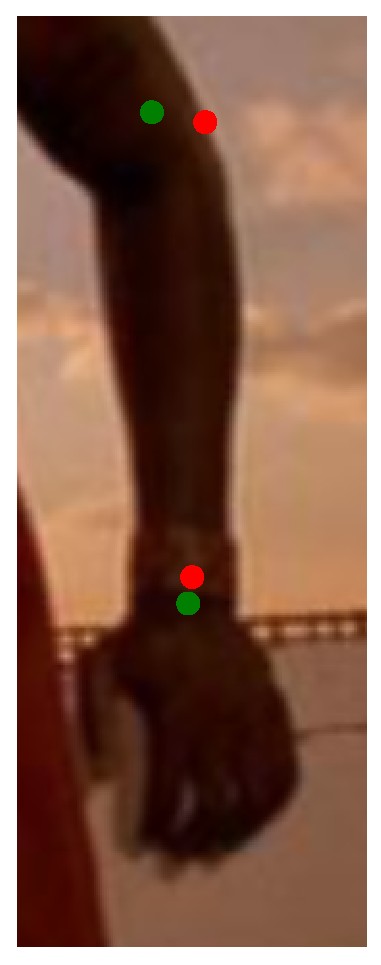
\includegraphics[height=0.3\columnwidth]{resources/Fixing/fix_14}
    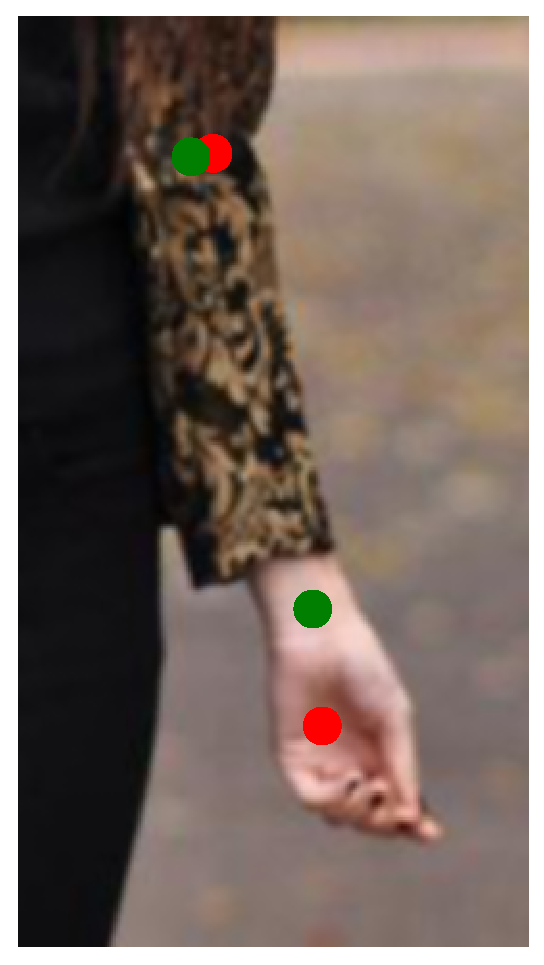
\includegraphics[height=0.3\columnwidth]{resources/Fixing/fix_15}
    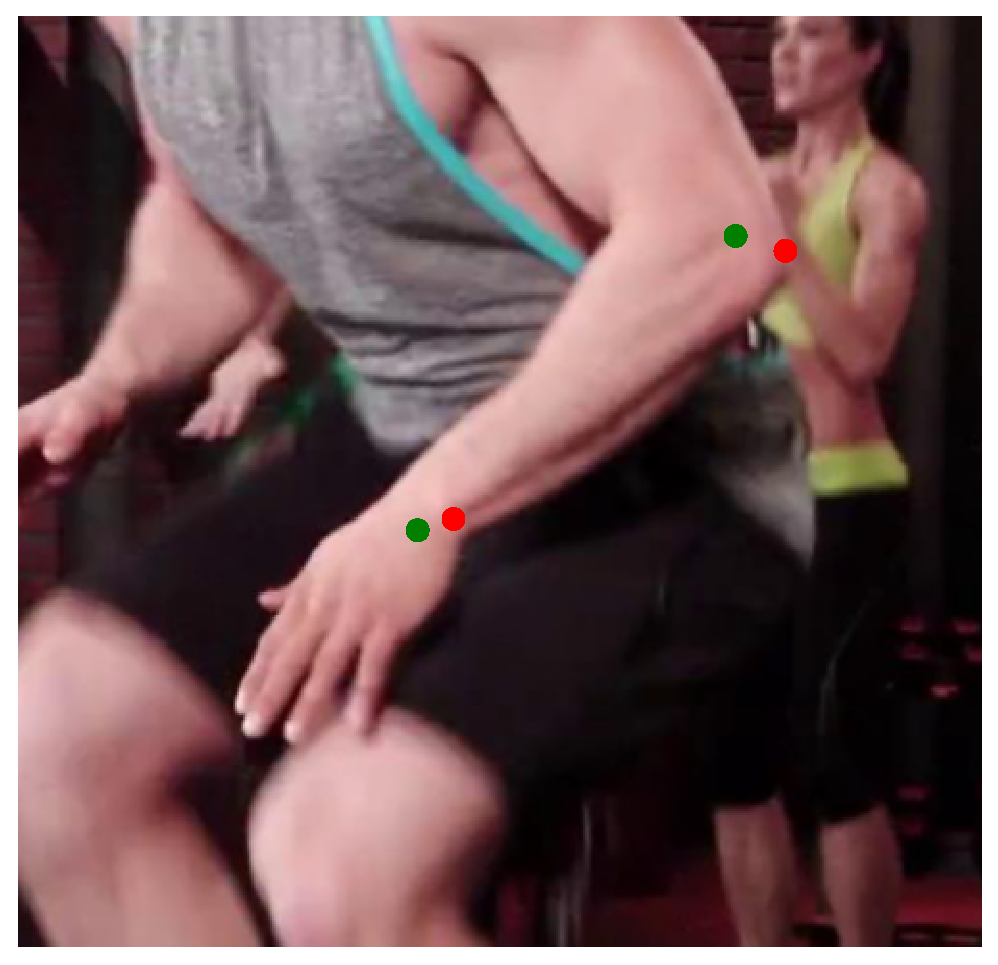
\includegraphics[height=0.3\columnwidth]{resources/Fixing/fix_17}
    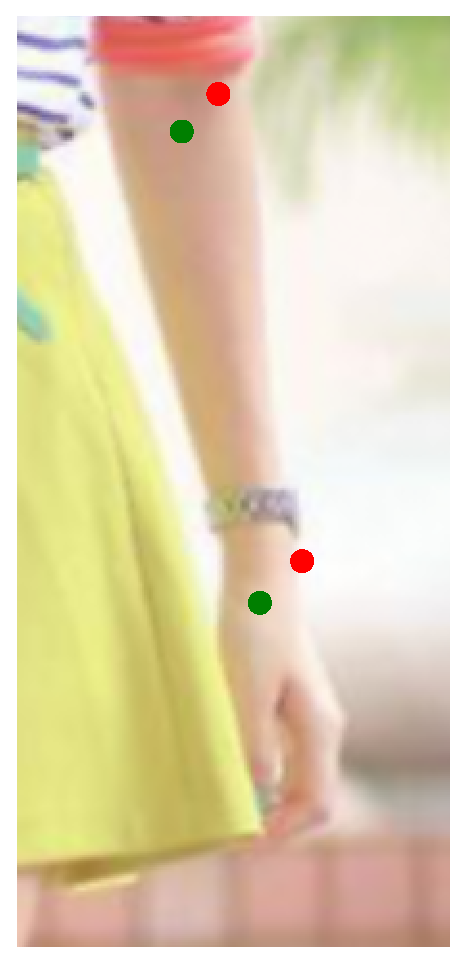
\includegraphics[height=0.3\columnwidth]{resources/Fixing/fix_18}
    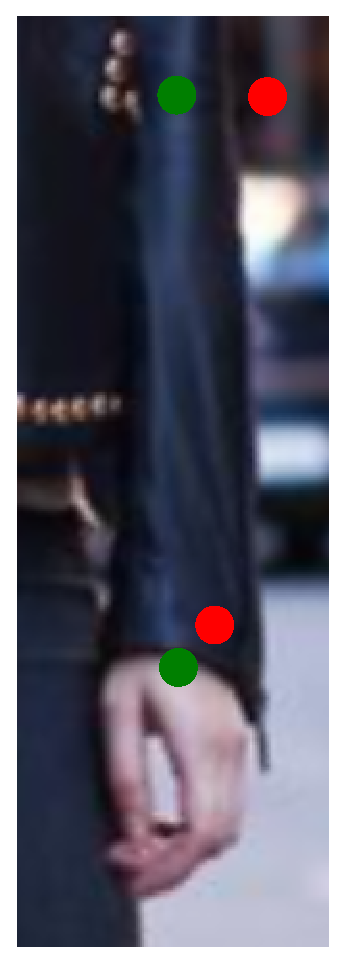
\includegraphics[height=0.3\columnwidth]{resources/Fixing/fix_19}
    \caption{CEDs of faces and ears fitting performance for experiment \ref{exp:daam_benchmark}}
    \label{fig:qualitative}
\end{figure}